\clearpage
\setcounter{page}{1}
\maketitlesupplementary
\appendix



This appendix provides further details, results, and analyses that could not be included in the main paper owing to space constraints. The content is organized as follows:
\begin{itemize}
    \item Sec.~\ref{sec:notation} provides the notation table for FedPuReL.
    \item Sec.~\ref{APP:Algorithm} presents the complete algorithm description.
    \item Sec.~\ref{app:additional_analysis} provides additional analysis of FedPuReL, including complementary branch contributions and gradient alignment dynamics.
    \item Sec.~\ref{app:Additional Experiments} presents further experimental results, including robustness to data heterogeneity, hyperparameter studies, and convergence analysis.
    \item Sec.~\ref{app:discussion} discusses the key insights and implications of FedPuReL.
\end{itemize}



\section{Notation Table}
\label{sec:notation}
We provide the notation table in Tab.~\ref{tab:notation}.

\begin{table}[ht]
\caption{Notation table for FedPuReL.}
\label{tab:notation}
\centering
\footnotesize
\resizebox{0.48\textwidth}{!}{
\setlength\tabcolsep{2.5pt}
\renewcommand\arraystretch{1.15}
\begin{tabular}{cl}
\hline\thickhline
\rowcolor{gray!20}
\textbf{Notation} & \textbf{Description} \\
\hline\hline
\multicolumn{2}{l}{\textcolor{gray!60}{\textit{Federated Learning Setup}}} \\
\cellcolor{gray!10}$K$ & \cellcolor{gray!10}Number of clients \\
$\mathcal{D}_k$ & Local dataset of client $k$ \\
\cellcolor{gray!10}$n_k$ & \cellcolor{gray!10}Number of samples in client $k$ \\
$\mathcal{S}_t$ & Set of selected clients at round $t$ \\
\cellcolor{gray!10}$C$ & \cellcolor{gray!10}Number of classes \\
$\mathrm{IF}$ & Imbalance factor ($n_1 / n_C$) \\
\cellcolor{gray!10}$\alpha_{\text{dir}}$ & \cellcolor{gray!10}Dirichlet parameter for heterogeneity \\
\hdashline
\multicolumn{2}{l}{\textcolor{gray!60}{\textit{Model Parameters}}} \\
\cellcolor{gray!10}$\boldsymbol{W}$ & \cellcolor{gray!10}Frozen CLIP backbone parameters \\
$\boldsymbol{\phi}_g$ & Global shared PEFT parameters \\
\cellcolor{gray!10}$\boldsymbol{\phi}_k$ & \cellcolor{gray!10}Personalized PEFT parameters for client $k$ \\
$f_{\text{img}}(\cdot)$, $f_{\text{text}}(\cdot)$ & Image and text encoders \\
\hdashline
\multicolumn{2}{l}{\textcolor{gray!60}{\textit{Predictions and Logits}}} \\
\cellcolor{gray!10}$\mathbf{x}$, $y$ & \cellcolor{gray!10}Input image and label \\
$\mathbf{z}(\mathbf{x})$ & Zero-shot logits \\
\cellcolor{gray!10}$\mathbf{f}(\mathbf{x})$ & \cellcolor{gray!10}Fine-tuned logits \\
$\mathbf{l}_{\text{G}}(\mathbf{x})$ & Global branch logits \\
\cellcolor{gray!10}$\mathbf{l}_{\text{P}}^k(\mathbf{x})$ & \cellcolor{gray!10}Personalized branch logits for client $k$ \\
\hdashline
\multicolumn{2}{l}{\textcolor{gray!60}{\textit{Metrics and Temperature}}} \\
\cellcolor{gray!10}$\tau$, $\tau_{zs}$, $\tau_{ft}$ & \cellcolor{gray!10}Temperature parameters \\
$D_{\text{TKL}}(\cdot \| \cdot)$ & Temperature-aligned KL divergence \\
\cellcolor{gray!10}$\beta(V)$ & \cellcolor{gray!10}Balancedness metric \\
$H(\cdot)$ & Entropy function \\
\hdashline
\multicolumn{2}{l}{\textcolor{gray!60}{\textit{Gradients and Losses}}} \\
\cellcolor{gray!10}$\mathbf{g}_{\text{task}}$ & \cellcolor{gray!10}Task gradient from cross-entropy loss \\
$\mathbf{g}_{\text{align}}$ & Alignment gradient from TKL divergence \\
\cellcolor{gray!10}$\tilde{\mathbf{g}}_{\text{task}}$ & \cellcolor{gray!10}Purified task gradient \\
$\mathcal{L}_{\text{align}}$ & Alignment loss \\
\cellcolor{gray!10}$\mathcal{L}_{\text{fusion}}^k$ & \cellcolor{gray!10}Fusion loss for additive combination \\
$\mathcal{L}_{\text{personal}}^k$ & Personalization loss \\
\cellcolor{gray!10}$\lambda$ & \cellcolor{gray!10}Weight balancing fusion and personal losses \\
\hline\thickhline
\end{tabular}
}
% \vspace{-10pt}
\end{table}


\section{Algorithm}
\label{APP:Algorithm}
We provide the algorithm description in Algorithm~\ref{alg:fedpurel}.

\begin{algorithm}[ht]
\caption{FedPuReL}
\label{alg:fedpurel}
\begin{algorithmic}[1]
\Require Number of clients $K$, global rounds $T$, personalization rounds $T_p$, balancedness weight $\lambda$, frozen CLIP weights $\boldsymbol{W}$.
\Ensure Global PEFT parameters $\boldsymbol{\phi}_g$, personalized parameters $\{\boldsymbol{\phi}_k\}_{k=1}^K$.

\State \textcolor{adaptive_blue}{\textbf{// Phase 1: Global Balanced Training}}
\State Initialize $\boldsymbol{\phi}_g^{(0)}$
\For{$t = 1, \ldots, T$}
  \State Select active clients $\mathcal{S}_t \subseteq [K]$
  \ForAll{client $k \in \mathcal{S}_t$ \textbf{in parallel}}
    \State Receive $\boldsymbol{\phi}_g^{(t)}$ from server
      \State Compute $\mathbf{z}(\mathbf{x})$, $\mathbf{f}(\mathbf{x}; \boldsymbol{W}, \boldsymbol{\phi}_g)$
      \State $\mathbf{g}_{\text{align}} \gets \nabla_{\boldsymbol{\phi}_g} D_{\text{TKL}}(\sigma_{\tau_{zs}}(\mathbf{z}) \| \sigma_{\tau_{ft}}(\mathbf{f}))$
      \State $\mathbf{g}_{\text{task}} \gets \nabla_{\boldsymbol{\phi}_g} \text{CE}(y, \sigma(\mathbf{f}))$
      \State \textbf{// Gradient Purification}
      \If{$\langle \mathbf{g}_{\text{task}}, \mathbf{g}_{\text{align}} \rangle < 0$}
        \State $\tilde{\mathbf{g}}_{\text{task}} \gets \mathbf{g}_{\text{task}} - \frac{\langle \mathbf{g}_{\text{task}}, \mathbf{g}_{\text{align}} \rangle}{\|\mathbf{g}_{\text{align}}\|^2} \mathbf{g}_{\text{align}}$
      \Else
        \State $\tilde{\mathbf{g}}_{\text{task}} \gets \mathbf{g}_{\text{task}}$
      \EndIf
      \State Update $\boldsymbol{\phi}_g$ with $\tilde{\mathbf{g}}_{\text{task}}$
    \State Upload $\boldsymbol{\phi}_g^{k,(t)}$ to server
  \EndFor
  \State $\boldsymbol{\phi}_g^{(t+1)} \gets \sum_{k \in \mathcal{S}_t} \frac{n_k}{\sum_{j \in \mathcal{S}_t} n_j} \boldsymbol{\phi}_g^{k,(t)}$
\EndFor

\State \textcolor{adaptive_blue}{\textbf{// Phase 2: Personalized Residual Learning}}
\State Freeze $\boldsymbol{\phi}_g^{(T)}$
\ForAll{client $k \in [K]$ \textbf{in parallel}}
  \State Initialize $\boldsymbol{\phi}_k$
  \For{$t_p = 1, \ldots, T_p$}
      \State $\mathbf{l}_{\text{G}} \gets f(\mathbf{x}; \boldsymbol{W}, \boldsymbol{\phi}_g^{(T)})$, $\mathbf{l}_{\text{P}}^k \gets f(\mathbf{x}; \boldsymbol{W}, \boldsymbol{\phi}_k)$
      \State $\mathcal{L}^k \gets (1-\lambda) \text{CE}(y, \sigma(\mathbf{l}_{\text{G}} + \mathbf{l}_{\text{P}}^k)) + \lambda \text{CE}(y, \sigma(\mathbf{l}_{\text{P}}^k))$
      \State Update $\boldsymbol{\phi}_k$ with $\nabla_{\boldsymbol{\phi}_k} \mathcal{L}^k$
    \EndFor
\EndFor
\State \Return $(\boldsymbol{W}, \boldsymbol{\phi}_g^{(T)})$, $\{(\boldsymbol{W}, \boldsymbol{\phi}_g^{(T)}, \boldsymbol{\phi}_k)\}_{k=1}^K$
\end{algorithmic}
\end{algorithm}








\section{Additional Analysis of FedPuReL}\label{app:additional_analysis}


\noindent \textbf{Analysis 4: Global and personalized branches exhibit complementary contributions.} 
Our design separates balanced global knowledge from personalized local adaptation, which should lead to different contribution patterns across class types. Specifically, head classes with abundant samples should rely more on global knowledge, while tail classes with scarce data should require stronger personalized corrections. 

To evaluate this, we decompose each correct prediction to identify the dominant contributor between the global and personalized branches. For each correctly classified sample $x$ with ground-truth label $y$, we compare the logits from both branches: $l_G^{(y)}(x)$ from the global branch and $l_P^{(y)}(x)$ from the personalized branch. We attribute the prediction to the branch with the higher logit value for the correct class, i.e., the prediction is attributed to the global branch if $l_G^{(y)}(x) > l_P^{(y)}(x)$, and to the personalized branch otherwise. We then compute the percentage of correct predictions attributed to each branch across all classes, grouped by their sample frequency.

As illustrated in Fig.~\ref{fig:any2}, as class frequency decreases from head to tail, the personalized branch contribution increases, while the global branch contribution decreases correspondingly. Notably, even for tail classes where personalization dominates, the global branch maintains a substantial 20-25\% contribution. These results confirm our design principle: the global branch provides consistent balanced knowledge across all classes, while the personalized branch dynamically adjusts its contribution to compensate for data scarcity.

\begin{figure}[ht]
\centering
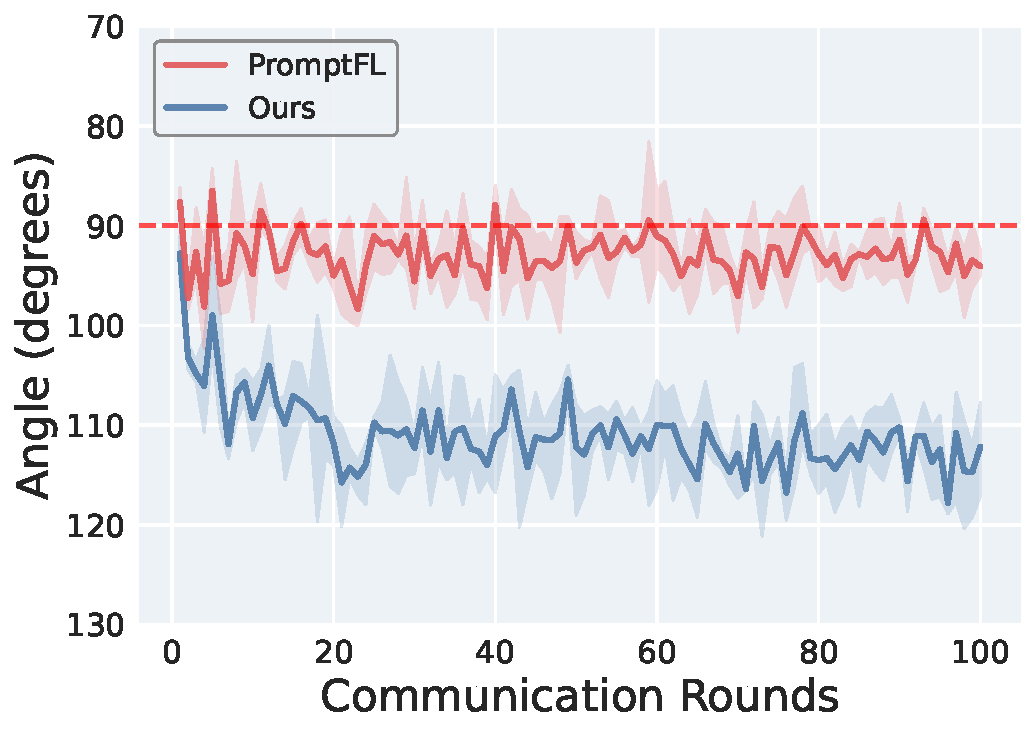
\includegraphics[width=0.7\linewidth]{fig/any1_gradient_angle_comparison_ci.pdf}
\caption{Angle between $\mathbf{g}_{\text{task}}$ and $\mathbf{g}_{\text{align}}$ during training on CIFAR-100-LT.}

\label{fig:gradient_angle}
% \vspace{-12pt}
\end{figure}



\noindent \textbf{Analysis 5: Gradient Alignment Dynamics.}
Fig.~\ref{fig:gradient_angle} visualizes the angle between task gradient $\mathbf{g}_{\text{task}}$ and alignment gradient $\mathbf{g}_{\text{align}}$ during training. Baseline methods exhibit convergence to approximately 90° (orthogonal), reflecting the well-known property that high-dimensional random vectors tend to be mutually orthogonal~\cite{cai2013distributions}. This orthogonality explains balance degradation, as task optimization proceeds without consideration of zero-shot alignment. In contrast, FedPuReL consistently maintains obtuse angles (\>90°), revealing that the original task gradient actively conflicts with balance preservation and would otherwise compromise zero-shot knowledge. Our purification operation detects these conflicts and removes incompatible components, ensuring updates remain aligned with balanced representations.



% \subsection{Discussion}
% FedPuReL introduces a conceptual shift, rather than explicitly rebalancing data or losses~\cite{wang2021ratioloss,sarkar2020fed}, we exploit the \textit{implicit balanced prior} in foundation models from large-scale pre-training. Gradient purification prevents erosion of this prior during adaptation, analogous to gradient projection in multi-task learning~\cite{yu2020gradient}, but with asymmetric priority favoring balance preservation. Residual learning at the logit level decouples personalization from representation, avoiding feature-level bias propagation~\cite{li2024fedotp,pan2024promptfolio} while enabling interpretable analysis of global-local complementarity (Sec.~\ref{Analysis of FedPuReL}, Analysis 4).




\section{Additional Experiments}
\label{app:Additional Experiments}


\begin{figure}[ht]
\centering
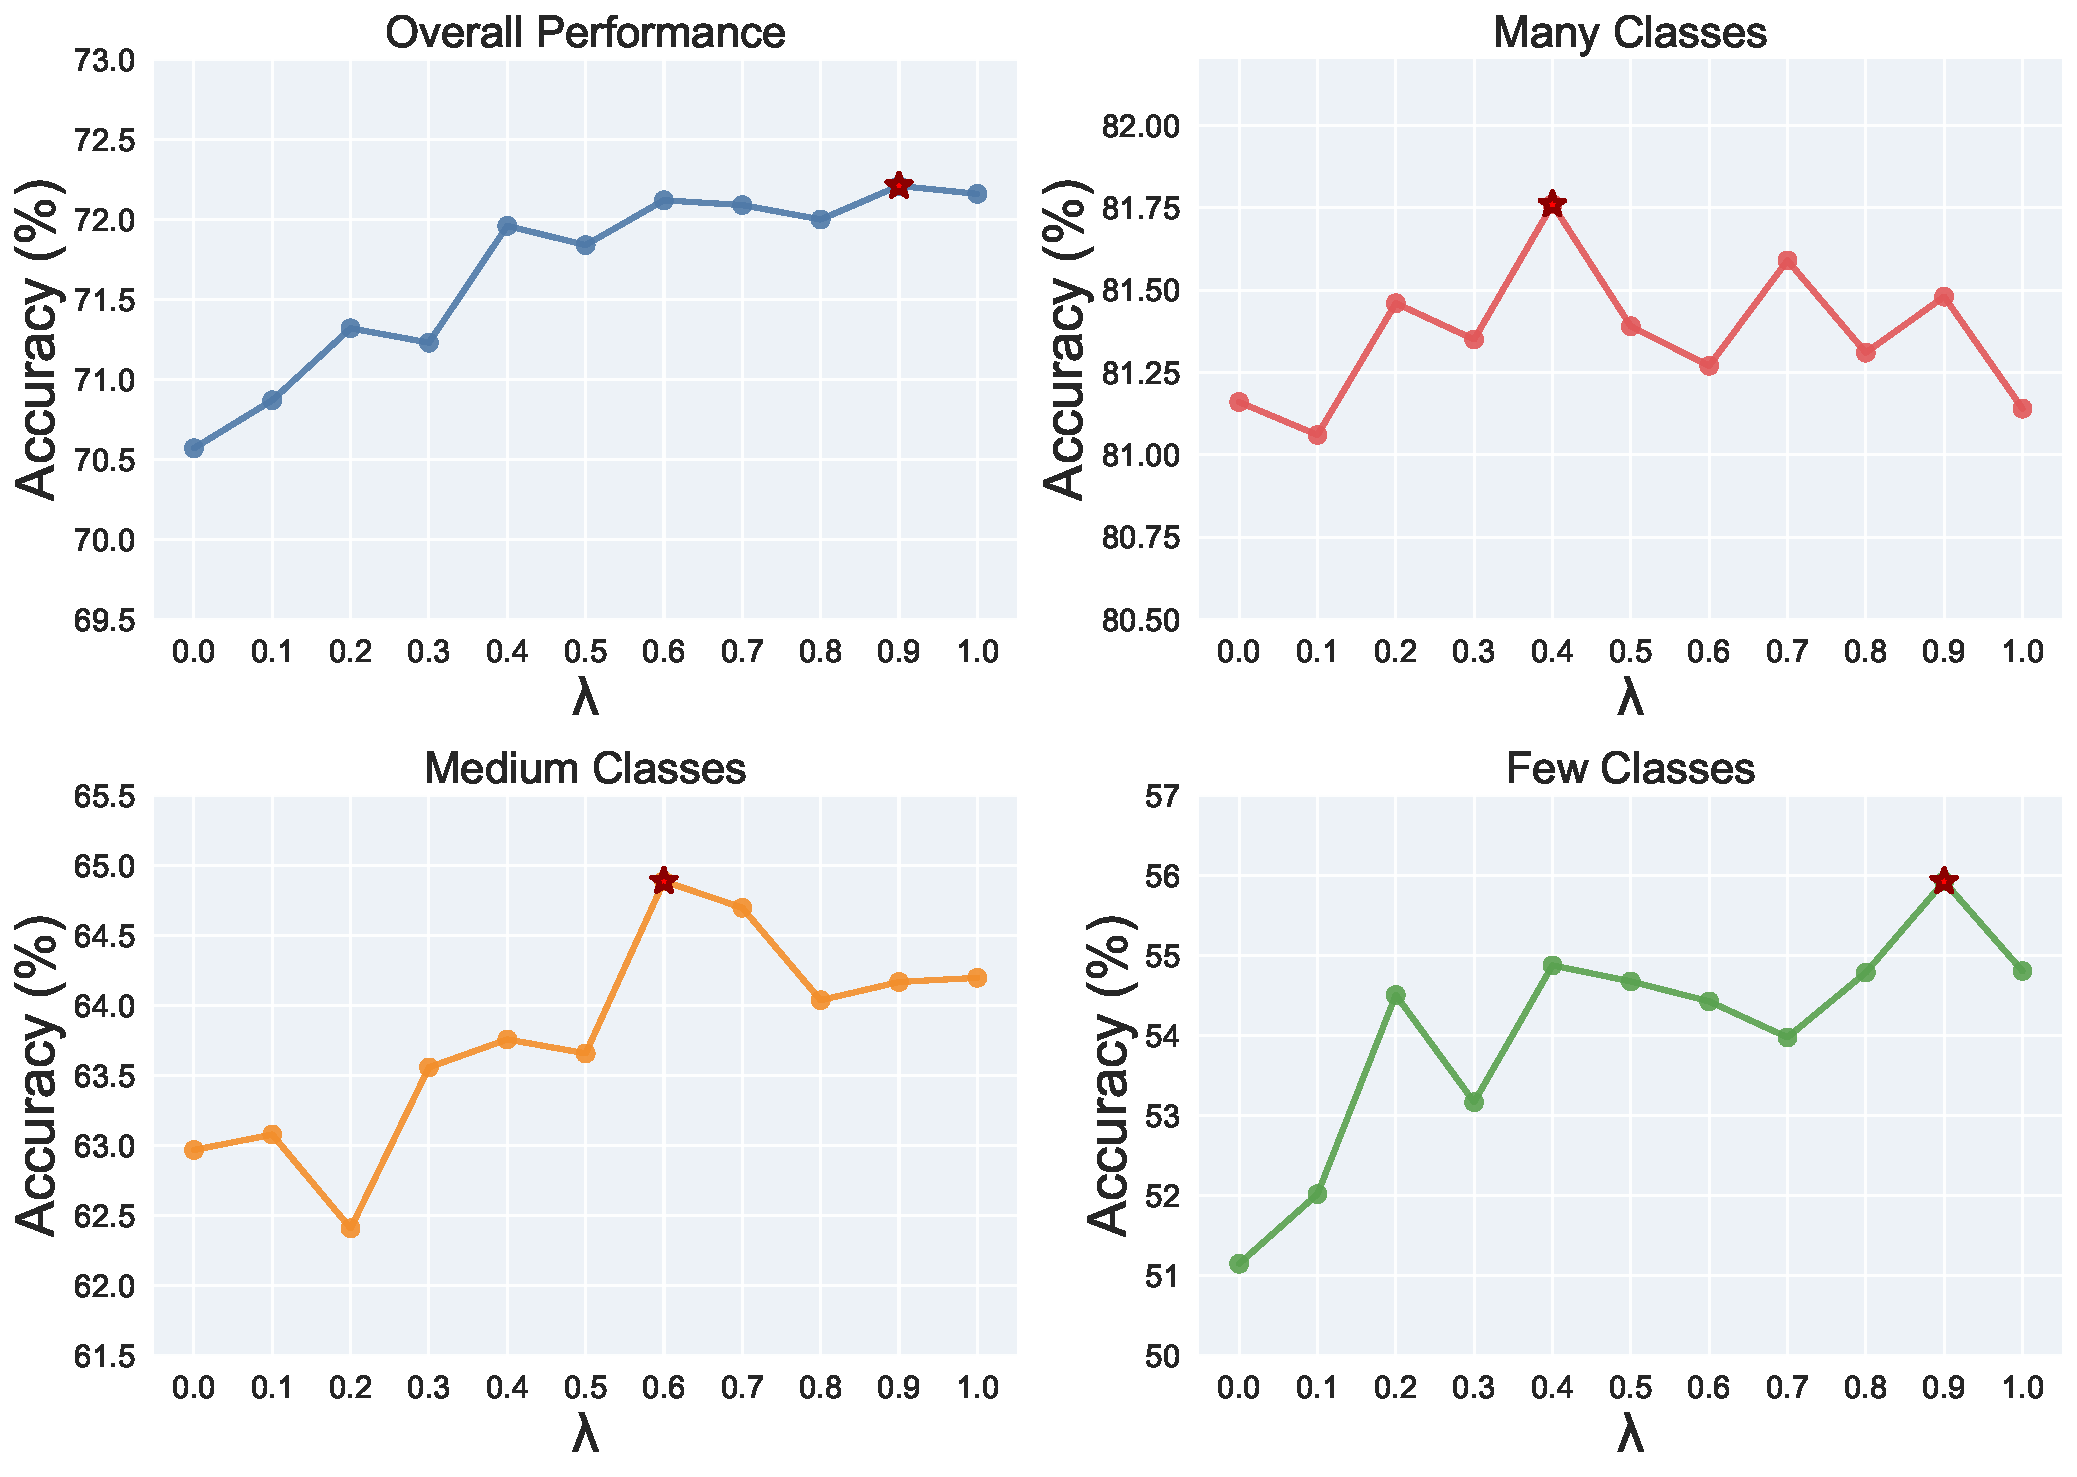
\includegraphics[width=\linewidth]{fig/ablation_lambda.pdf}
\caption{\textbf{Ablation study on $\lambda$ in Eq.~\ref{fusion loss}.} Performance across overall, Head, Mid, and Tail classes on CIFAR-100-LT with varying $\lambda$ values. Red stars mark optimal points.}
\label{fig:ablation_lambda}
\end{figure}


\begin{figure}[!t]
\centering
\begin{subfigure}[b]{\linewidth}
    \centering
    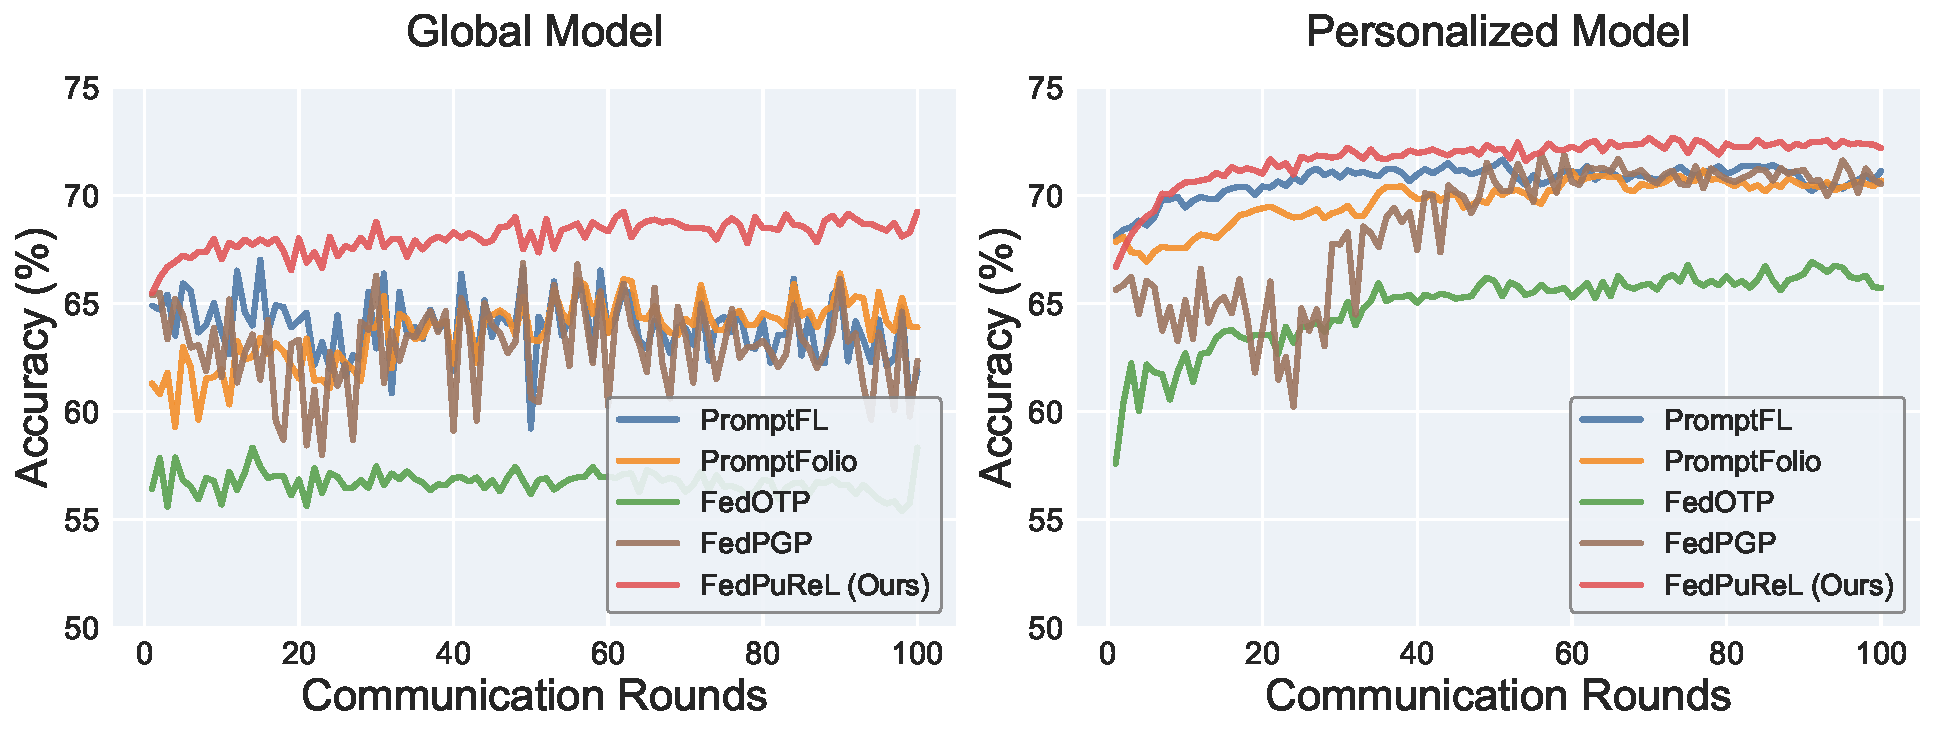
\includegraphics[width=\linewidth]{fig/all_methods_overall.pdf}
    \caption*{(a) Overall Accuracy}
\end{subfigure}
\hfill
\begin{subfigure}[b]{\linewidth}
    \centering
    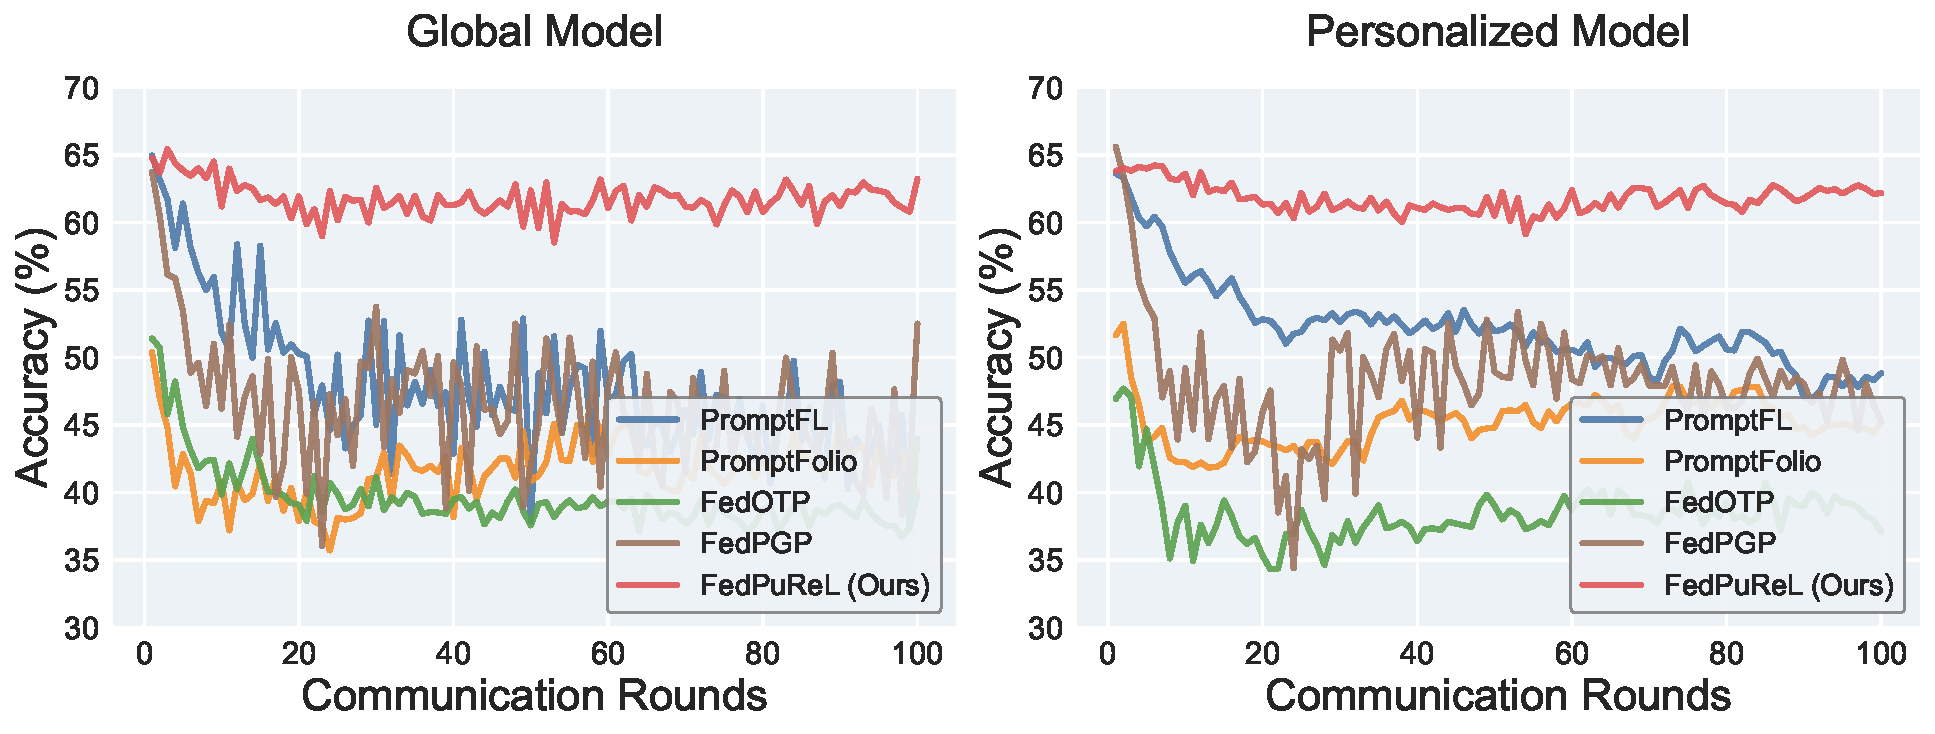
\includegraphics[width=\linewidth]{fig/tail_class_accuracy.pdf}
    \caption*{(b) Few Class Accuracy}
\end{subfigure}
\vspace{-0.5em}
\caption{\textbf{Convergence of average accuracy} compared to Prompt-based SOTA method on CIAFR-100-LT}
\label{fig:acc_trend}
\end{figure}

\noindent \textbf{Ablation of TKL vs.\ Standard KL.}
Fig.~6 in the main paper qualitatively demonstrates that TKL distinguishes balanced adaptation from biased divergence, whereas standard KL exhibits large values even on balanced data due to confidence shifts.
To further validate this quantitatively, we replace TKL with standard KL divergence in the gradient purification module and evaluate on CIFAR-100-LT.
As shown in Table~\ref{tab:tkl_ablation}, TKL consistently outperforms standard KL in both accuracy and balancedness across global and personalized settings.
This confirms that temperature alignment is essential for isolating structural distributional shift from benign confidence growth during fine-tuning, enabling more effective gradient purification.

\begin{table}[ht]
\caption{\textbf{Ablation of TKL vs.\ standard KL} on CIFAR-100-LT.}
\label{tab:tkl_ablation}
\centering
\footnotesize
\setlength\tabcolsep{4pt}
\renewcommand\arraystretch{1.15}
\begin{tabular}{r||cc|cc}
\hline\thickhline
\rowcolor{gray!20}
 & \multicolumn{2}{c|}{\textbf{Accuracy (\%)}} & \multicolumn{2}{c}{\textbf{Balancedness (\%)}} \\
\cline{2-5}
\rowcolor{gray!20}
\textbf{Metric} & \textbf{GM} & \textbf{PM} & \textbf{GM} & \textbf{PM} \\
\hline\hline
\cellcolor{gray!10} KL & \cellcolor{gray!10} 67.92 & \cellcolor{gray!10} 71.62 & \cellcolor{gray!10} 25.03 & \cellcolor{gray!10} 27.84 \\
\cellcolor[HTML]{D7F6FF}\textbf{TKL (ours)} & \cellcolor[HTML]{D7F6FF}\textbf{69.77} & \cellcolor[HTML]{D7F6FF}\textbf{73.37} & \cellcolor[HTML]{D7F6FF}\textbf{27.87} & \cellcolor[HTML]{D7F6FF}\textbf{30.02} \\
\hline\thickhline
\end{tabular}
\vspace{-8pt}
\end{table}


\noindent \textbf{Robustness to Data Heterogeneity.} We evaluate FedPuReL's robustness across varying degrees of client heterogeneity by adjusting the Dirichlet parameter $\alpha \in \{0.1, 0.5, 1, 5\}$, where smaller $\alpha$ indicates higher non-IID heterogeneity. As shown in Table~\ref{tab:cifar100_lt_alpha}, FedPuReL consistently outperforms all baselines across different heterogeneity levels in both global and personalized settings. This robustness stems from our gradient purification mechanism, which anchors local updates to the zero-shot foundation model, effectively preventing divergence caused by heterogeneous local distributions. The consistent performance across all $\alpha$ values demonstrates that FedPuReL successfully preserves balanced knowledge while adapting to diverse client-specific distributions.

\noindent \textbf{Hyperparameter Study.} We analyze the impact of the balancing coefficient $\lambda$ in Eq.~\ref{fusion loss}, which controls the trade-off between fusion loss $\mathcal{L}^k_{\text{fusion}}$ and personalization loss $\mathcal{L}^k_{\text{personal}}$. As shown in Fig.~\ref{fig:ablation_lambda}, we observe that $\lambda$ exhibits different optimal values across class groups: $\lambda=0.9$ achieves the best overall and tail class performance, while moderate values favor head and mid classes. This demonstrates that higher $\lambda$ values, which emphasize the personalized branch, are particularly beneficial for tail classes that require stronger client-specific corrections. Notably, head classes maintain relatively stable performance across different $\lambda$ values, benefiting from the robust global branch. We set $\lambda=0.9$ as the default in our experiments to balance overall accuracy with tail class performance.

\noindent \textbf{Model Convergence Analysis.} Fig.~\ref{fig:acc_trend} visualizes the training dynamics of FedPuReL compared to state-of-the-art prompt-based methods on CIFAR-100-LT. For overall accuracy (Fig.~\ref{fig:acc_trend}a), FedPuReL maintains stable performance throughout training in both global and personalized settings. In contrast, baseline methods exhibit significant fluctuations and fail to achieve comparable performance. More critically, for few-shot class accuracy (Fig.~\ref{fig:acc_trend}b), FedPuReL maintains consistently superior performance on tail classes, while baselines show severe degradation or instability. This stability stems from our gradient purification mechanism, which prevents the model from drifting away from the balanced zero-shot anchor during adaptation. The consistent gap between FedPuReL and baselines throughout training validates that preserving balanced knowledge is essential for sustained performance on long-tailed federated data.




\begin{table}[ht]\footnotesize
\caption{\textbf{Comparison with state-of-the-art methods} on CIFAR-100-LT under different degrees of data heterogeneity ($\alpha$) for global models (GM) and personalized models (PM).}
\centering
\scriptsize{
\resizebox{\linewidth}{!}{
\setlength\tabcolsep{1.5pt}
\renewcommand\arraystretch{1.1}
\begin{tabular}{r||cc|cc|cc|cc}
\cline{2-9}
\hline\thickhline
\rowcolor{gray!20}
\textbf{CIFAR-100-LT} &
  \multicolumn{2}{c|}{\textbf{$\alpha = 0.1$}} &
  \multicolumn{2}{c|}{\textbf{$\alpha = 0.5$}} &
  \multicolumn{2}{c|}{\textbf{$\alpha = 1$}} &
  \multicolumn{2}{c}{\textbf{$\alpha = 5$}} \\
\cline{2-9}
\rowcolor{gray!20}
\textbf{Method} & \textbf{GM} & \textbf{PM} & \textbf{GM} & \textbf{PM} & \textbf{GM} & \textbf{PM} & \textbf{GM} & \textbf{PM} \\
\hline\hline
Zero-shot & 64.82 & 64.79 & 64.82 & 64.79 & 64.82 & 64.79 & 64.82 & 64.79 \\
\hdashline
\multicolumn{9}{l}{\textcolor{gray!60}{\textit{Prompt-based}}} \\
\cellcolor{gray!10}PromptFL~\cite{guo2023promptfl}
 & \cellcolor{gray!10}63.72 & \cellcolor{gray!10}72.18 & \cellcolor{gray!10}65.25 & \cellcolor{gray!10}71.97 & \cellcolor{gray!10}61.98 & \cellcolor{gray!10}70.52 & \cellcolor{gray!10}64.95 & \cellcolor{gray!10}71.38 \\
PromptFolio~\cite{pan2024promptfolio}
 & 64.32 & 72.83 & 64.79 & 72.19 & 64.10 & 70.54 & 65.68 & 71.10 \\
\cellcolor{gray!10}FedOTP~\cite{li2024fedotp}
 & \cellcolor{gray!10}57.27 & \cellcolor{gray!10}70.87 & \cellcolor{gray!10}55.75 & \cellcolor{gray!10}68.28 & \cellcolor{gray!10}58.02 & \cellcolor{gray!10}65.23 & \cellcolor{gray!10}54.88 & \cellcolor{gray!10}65.77 \\
FedPGP~\cite{cui2024fedpgp}
 & 61.66 & 73.10 & 62.12 & 72.56 & 62.96 & 67.83 & 63.41 & 70.41 \\
 PromptFolio+Fed-GraB~\cite{Fed-Grab}
 & \underline{64.97} & \underline{75.13} & \underline{65.43} & \underline{73.26} & \underline{65.14} & \underline{71.79} & \underline{66.23} & \underline{72.18} \\
 
\cellcolor[HTML]{D7F6FF}\textbf{FedPuReL (ours)}
 & \cellcolor[HTML]{D7F6FF}\textbf{68.88} & \cellcolor[HTML]{D7F6FF}\textbf{77.72} & \cellcolor[HTML]{D7F6FF}\textbf{69.05} & \cellcolor[HTML]{D7F6FF}\textbf{74.97} & \cellcolor[HTML]{D7F6FF}\textbf{69.77} & \cellcolor[HTML]{D7F6FF}\textbf{73.37} & \cellcolor[HTML]{D7F6FF}\textbf{70.54} & \cellcolor[HTML]{D7F6FF}\textbf{73.71} \\
 % ===== Prompt-based: Δ row (FedPuReL - best baseline) =====
\textcolor{gray!60}&
\blueup{3.91} & \blueup{2.59} &
\blueup{3.62} & \blueup{1.71} &
\blueup{4.63} & \blueup{1.58} &
\blueup{4.31} & \blueup{1.53} \\
\hline
\multicolumn{9}{l}{\textcolor{gray!60}{\textit{LoRA-based}}} \\
CLIPLoRA~\cite{cliplora}
 & 74.83 & 78.53 & 75.50 & 78.75 & 75.02 & 77.80 & 76.12 & 79.12 \\
FedSA-LoRA~\cite{wang2024fedsalora}
 & 73.53 & \underline{80.47} & 73.41 & \underline{79.16} & 74.48 & \underline{81.68} & 73.03 & 76.91 \\
 CLIPLoRA+Fed-GraB~\cite{Fed-Grab}
 & \underline{75.30} & 79.12 & \underline{76.43} & 78.97 & \underline{76.35} & 77.91 & \underline{77.31} & \underline{79.62} \\
 
\cellcolor[HTML]{D7F6FF}\textbf{FedPuReL (ours)}
 & \cellcolor[HTML]{D7F6FF}\textbf{76.71} & \cellcolor[HTML]{D7F6FF}\textbf{81.76} & \cellcolor[HTML]{D7F6FF}\textbf{76.74} & \cellcolor[HTML]{D7F6FF}\textbf{80.29} & \cellcolor[HTML]{D7F6FF}\textbf{77.56} & \cellcolor[HTML]{D7F6FF}\textbf{84.62} & \cellcolor[HTML]{D7F6FF}\textbf{78.20} & \cellcolor[HTML]{D7F6FF}\textbf{80.27} \\
 % ===== LoRA-based: Δ row (FedPuReL - best baseline) =====
\textcolor{gray!60} &
\blueup{1.41} & \blueup{1.29} &
\blueup{0.31} & \blueup{1.13} &
\blueup{1.21} & \blueup{2.94} &
\blueup{0.89} & \blueup{0.65} \\

\hline
\multicolumn{9}{l}{\textcolor{gray!60}{\textit{Adapter-based}}} \\
FedClip~\cite{lu2023fedclip}
 & 63.92 & 68.02 & 64.54 & 68.64 & 64.09 & 66.87 & 64.35 & 68.19 \\

 FedClip+Fed-GraB~\cite{Fed-Grab}
 & \underline{64.69} & \underline{68.18} & \underline{65.72} & \underline{68.98} & \underline{65.40} & \underline{67.20} & \underline{66.02} & \underline{68.49} \\
 
\cellcolor[HTML]{D7F6FF}\textbf{FedPuReL (ours)}
 & \cellcolor[HTML]{D7F6FF}\textbf{66.58} & \cellcolor[HTML]{D7F6FF}\textbf{68.98} & \cellcolor[HTML]{D7F6FF}\textbf{66.83} & \cellcolor[HTML]{D7F6FF}\textbf{69.38} & \cellcolor[HTML]{D7F6FF}\textbf{67.54} & \cellcolor[HTML]{D7F6FF}\textbf{68.42} & \cellcolor[HTML]{D7F6FF}\textbf{67.81} & \cellcolor[HTML]{D7F6FF}\textbf{69.05} \\
 % ===== Adapter-based: Δ row (FedPuReL - best baseline) =====
\textcolor{gray!60}&
\blueup{1.89} & \blueup{0.80} &
\blueup{1.11} & \blueup{0.40} &
\blueup{2.14} & \blueup{1.22} &
\blueup{1.79} & \blueup{0.56} \\

% \hline\thickhline
\end{tabular}}
}
\vspace{-12pt}
\label{tab:cifar100_lt_alpha}
\end{table}



\section{Discussion}\label{app:discussion}
FedPuReL preserves balanced knowledge in foundation models while enabling effective personalization. Gradient purification maintains balancedness close to zero-shot model throughout training (cf. Analysis~\hyperlink{analysis:1}{1} in Sec. 4.5). Residual learning then enables unbiased personalization through output-space offsets: Analysis~\hyperlink{analysis:4}{4} reveals complementary contributions where the global branch provides consistent knowledge across all classes while the personalized branch dynamically compensates for data scarcity in tail classes. Additionally, unlike methods requiring explicit class priors~\cite{zhang2024rucr,Fed-Grab}, our approach leverages implicit balanced priors in foundation models, eliminating the need for class distribution that pose privacy risks while exceeding prior-based performance (Sec.~\ref{Comparison with State-of-the-Art}). By reducing distributional divergence and client drift (Analysis~\hyperlink{analysis:2}{2}--\hyperlink{analysis:3}{3}), FedPuReL achieves superior convergence without explicit rebalancing.